\documentclass{article}

\title{beautier: BEAUti for R}
\author{Rich\`el J.C. Bilderbeek, Rampal S. Etienne}

\usepackage{listings}
\usepackage{hyperref}
\usepackage{todonotes}
\usepackage{verbatim}
\usepackage{tikz}
\usepackage{tkz-graph}
\usepackage{pgf}
\usetikzlibrary{arrows,automata}

% Style of listings
% From http://r.789695.n4.nabble.com/How-to-nicely-display-R-code-with-the-LaTeX-package-listings-tp4648110.html
\usepackage{fancyvrb} 
\definecolor{codegreen}{rgb}{0,0.6,0}
\definecolor{codegray}{rgb}{0.5,0.5,0.5}
\definecolor{codepurple}{rgb}{0.58,0,0.82}
\definecolor{backcolor}{rgb}{0.95,0.95,0.92}
\lstdefinestyle{mystyle}{
  language=R,% set programming language
  basicstyle=\ttfamily\small,% basic font style
  commentstyle=\color{gray},% comment style
  numbers=left,% display line numbers on the left side
  numberstyle=\scriptsize,% use small line numbers
  numbersep=10pt,% space between line numbers and code
  tabsize=2,% sizes of tabs
  showstringspaces=false,% do not replace spaces in strings by a certain character
  captionpos=b,% positioning of the caption below
  breaklines=true,% automatic line breaking
  escapeinside={(*}{*)},% escaping to LaTeX
  fancyvrb=true,% verbatim code is typset by listings
  extendedchars=false,% prohibit extended chars (chars of codes 128--255)
  literate={"}{{\texttt{"}}}1{<-}{{$\bm\leftarrow$}}1{<<-}{{$\bm\twoheadleftarrow$}}1
  {~}{{$\bm\sim$}}1{<=}{{$\bm\le$}}1{>=}{{$\bm\ge$}}1{!=}{{$\bm\neq$}}1{^}{{$^{\bm\wedge}$}}1,% item to replace, text, length of chars
  alsoletter={.<-},% becomes a letter
  alsoother={$},% becomes other
  otherkeywords={!=, ~, $, \&, \%/\%, \%*\%, \%\%, <-, <<-, /},% other keywords
  deletekeywords={c}% remove keywords 
}
\lstset{style=mystyle}

% Adds numbered lines, thanks to Raphael Scherrer
% \usepackage[switch]{lineno}



\begin{document}

\maketitle

% TODO: RS: Rename to 'Summary 
% https://tex.stackexchange.com/a/24778 does not work:
% \addto{\captionsenglish}{\renewcommand{\abstractname}{Summary}}

\begin{abstract}

  \textbf{1. }
    In the field of phylogenetics, 
     BEAST2 is one of the most widely used software tools. 
     It comes with the graphical program BEAUti to 
     facilitate the creation of input files to BEAST2. 
     However, when many input files are needed, 
     such a GUI is cumbersome. 
     Moreover, many other phygenetics tools are available 
     in R, which requires switching from one platform 
     to the other. \\
  \textbf{2. }
    Here, we present a free, libre and open-source package, \verb;beautier;, 
    'BEAUti for R', for the R programming language. 
    \verb;beautier; creates BEAST2 input files 
    from an R function call. \\
  \textbf{3. }
    We describe \verb;beautier;'s usage, the novel functionality it provides
    compared to BEAUti, and give some examples. \\
  \textbf{4. }
    As \verb;beautier; is designed to be of high quality and extendable, 
    we conclude by describing the further development of the package \\
\end{abstract}

% TODO: RS: Get these keywords visualized
% Key-words: computational biology, evolution, phylogeny, BEAST2, R

%%%%%%%%%%%%%%%%%%%%%%%%%%%%%%%%%%%%%%%%%%%%%%%%%%%%%%%%%%%%%%%%%%%%%%%%%%%%%%%%%%%%%%
\section{Introduction}
%%%%%%%%%%%%%%%%%%%%%%%%%%%%%%%%%%%%%%%%%%%%%%%%%%%%%%%%%%%%%%%%%%%%%%%%%%%%%%%%%%%%%%

Phylogenies are commonly used to explore evolutionary hypotheses.
Not only can phylogenies show us how species (or other
evoliutionary units) relate to each other, 
but also relevant parameters like extinction and 
speciation rates can be estimated from them.


There are many phylogenetics tools available to obtain an estimate 
of the phylogenetic tree of a given set of species. 
BEAST2 \cite{bouckaert2014beast} is one of the most widely used ones. 
It creates a posterior of jointly-estimated phylogenies and model parameters, 
from a DNA, RNA or amino acid alignment (see figure \ref{fig:workflow} 
for an overview of the workflow). 
It is a console application, that needs a configuration file containing alignments and model parameters.

BEAST2 is bundled with BEAUti 2 \cite{drummond2012bayesian} ('BEAUti' from now on), 
a desktop application to create a BEAST2 configuration file.
BEAUti has a user-friendly graphical user interface, with helpful and reasonable default settings.
As such, BEAUti is an attractive alternative 
to manual and error-prone editing of BEAST2 configuration files. 

BEAUti cannot be called from a command-line script.
This implies that when the user 
wants to explore the consequences of various settings, this must be done manually.
This is the common workflow when using a few alignments and doing a superficial 
analysis of sensitivity of the reconstructed tree to model settings. 

However, for exploring many trees (for instance from simulations) and for
more thorough sensitivity analysis, one would like to loop through 
multiple (simulated) alignments, nucleotide substitution models, 
clock models and tree priors. 

Here, to provide such functionality we present \verb;beautier;, 
’BEAUti for R’, which creates BEAST2 configuration files 
from an R function call and hence
will save time and tedious mouse clicking and 
reduces the chances of errors in such repetitive actions.
The interface of \verb;beautier; mimics BEAUti. This
familiarity helps both beginner and experienced BEAST2 users 
to create configuration files using \verb;beautier;.
Because there are many R packages for exploring the 
resulting phylogenetic trees, 
\verb;beautier; enables the creation of a single-script 
pipeline from sequence alignments to tree analysis in R. 

\verb;beautier; has a similar goal as \verb;BEASTmasteR; \cite{beastmaster} (still
in pre-release), as both
allow for scripted use of BEAST2. The difference is that \verb;beautier; 
has its focus on DNA alignments and ultrametric trees, 
where \verb;BEASTmasteR; is used for 
morphologucal traits and tip-dating. 

%%%%%%%%%%%%%%%%%%%%%%%%%%%%%%%%%%%%%%%%%%%%%%%%%%%%%%%%%%%%%%%%%%%%%%%%%%%%%%%%
\begin{figure}
  \centering
  \begin{tikzpicture}[->,>=stealth',shorten >=1pt,auto,node distance=6cm, semithick]   
  \tikzstyle{every state}=[]
  \node[state] (A) [rectangle] {
    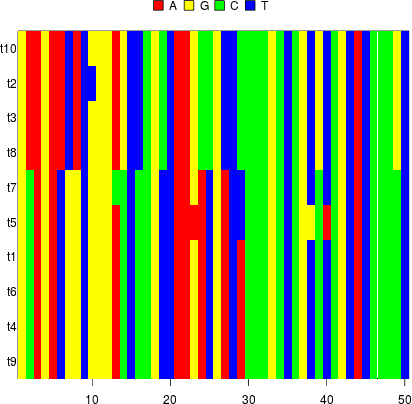
\includegraphics[width=0.2\textwidth]{alignment.png}
    
\includegraphics[width=0.2\textwidth]{thought_cloud.png}
  };   
  \node[state] (E) [below of=A, rectangle] {
    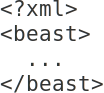
\includegraphics[height=0.1\textheight]{xml.png}
  };   
  \node[state] (F) [rectangle, below of=E] {
    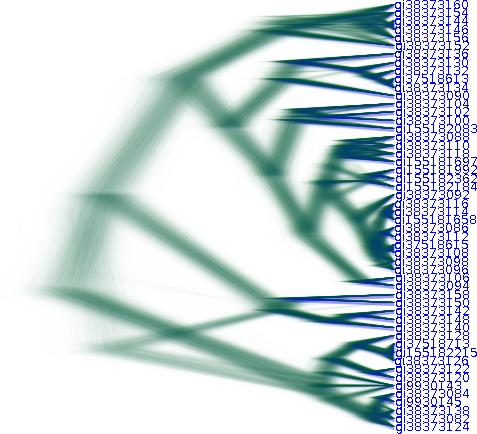
\includegraphics[width=0.3\textwidth]{DensiTreeExample2.jpg}
    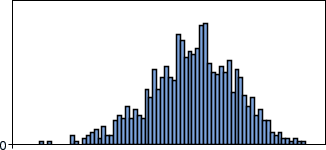
\includegraphics[width=0.6\textwidth]{ParameterEstimates.png}
  };
  \path (A) edge [anchor = east] node {
\includegraphics[height=0.15\textheight]{beautier_logo.png}} (E)
        (A) edge [anchor = west] node {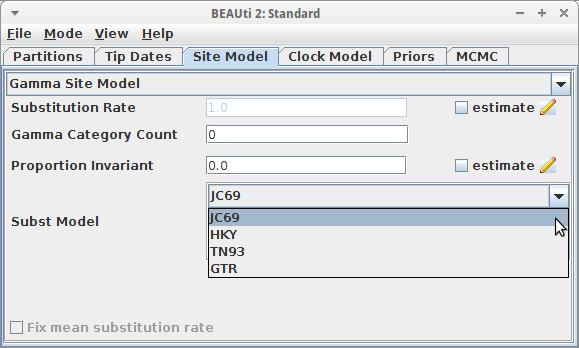
\includegraphics[height=0.15\textheight]{BeautiSiteModel.png}} (E)
        % (E) edge [anchor = east] node {
\includegraphics[width=0.25\textwidth]{lumier_logo_big.png}} (F) 
        (E) edge [anchor = west] node {
\includegraphics[width=0.2\textwidth]{beast_logo.png}} (F); 
  \end{tikzpicture}

  \caption{
    Workflow. From an alignment and priors (depicted as a thought cloud), one creates a BEAST2 XML input file. This
    can be done using beautier or BEAUti. The created configuration file is run by BEAST2
    to create a posterior of phylogenies and model parameter estimates.
  }
  \label{fig:workflow}
\end{figure}
%%%%%%%%%%%%%%%%%%%%%%%%%%%%%%%%%%%%%%%%%%%%%%%%%%%%%%%%%%%%%%%%%%%%%%%%%%%%%%%%

%%%%%%%%%%%%%%%%%%%%%%%%%%%%%%%%%%%%%%%%%%%%%%%%%%%%%%%%%%%%%%%%%%%%%%%%%%%%%%%%%%%%%%
\section{Description}
%%%%%%%%%%%%%%%%%%%%%%%%%%%%%%%%%%%%%%%%%%%%%%%%%%%%%%%%%%%%%%%%%%%%%%%%%%%%%%%%%%%%%%

\verb;beautier; is written in the R programming language \cite{R}
and creates a BEAST2 configuration file from an R function call,
in a similar way that BEAUti does.

\verb;beautier;'s main function is \verb;create_beast2_input_file;, which, 
as the name suggests, creates a BEAST2 configuration file. 
\verb;create_beast2_input_file; needs at least the name of a 
FASTA file containing a DNA alignment
and a name for the to-be-created configuration file. 
The default settings for the other arguments of \verb;create_beast2_input_file; 
are identical to BEAUti's default settings.
Per alignment, a site model, clock model and tree prior can be chosen.
Multiple alignments can be used, each with its own (unlinked) site model, clock model and tree prior.

\verb;beautier; currently has 61 exported functions to create a BEAST2 configuration file. 
\verb;beautier; is an alternative for a majority of BEAUti use cases, 
but does not yet support the full functionality of BEAUti. 
Because of BEAUti's high number of plugins, 
\verb;beautier; uses a software architecture that expects te be extended.

\verb;beastier; \cite{beastier} and \verb;lumier; \cite{lumier} are related packages, used to confirm the correct working of verb;beautier;.
\verb;lumier; calls BEAST2 from within R and is used to confirm that the XML files created by \verb;beautier; are valid. 
Additionally, \verb;lumier; is used to run BEAST2 to create posteriors. 
\verb;beastier; can parse BEAST2 posteriors, and is used to confirm whether posteriors have an estimated or fixed crown age.

%%%%%%%%%%%%%%%%%%%%%%%%%%%%%%%%%%%%%%%%%%%%%%%%%%%%%%%%%%%%%%%%%%%%%%%%%%%%%%%%%%%%%%
\section{Examples}
%%%%%%%%%%%%%%%%%%%%%%%%%%%%%%%%%%%%%%%%%%%%%%%%%%%%%%%%%%%%%%%%%%%%%%%%%%%%%%%%%%%%%%

In R, the functions of a package need to be loaded in the global namespace first:

\begin{lstlisting}[language=R, caption=Loading, label=lst:loading_beautier, floatplacement=H]
library(beautier)
\end{lstlisting}

BEAUti, and likewise \verb;beautier;, needs at least a FASTA filename
and an output filename. In BEAUti, this is achieved by loading a FASTA file, 
then saving an output file using a common
save file dialog. In \verb;beautier;, the same is achieved by:

\begin{lstlisting}[language=R, caption=Simplest example, label=lst:simplest_example, floatplacement=H]
create_beast2_input_file(
  "alignment.fas",
  "beast2.xml"
)
\end{lstlisting}

This code will create a BEAST2 configuration file with name '\verb;beast2.xml;',
using a FASTA file with name \verb;alignment.fas;, using the same default settings as BEAUti.
The default settings are, among others, to use a Jukes-Cantor site model \cite{cantor1969mammalian}, 
a strict clock, and a Yule birth tree prior \cite{yule}. 

An example of using a different site model, clock model 
and tree prior is:

\begin{lstlisting}[language=R, caption=Example with different site model and clock model and tree prior, label=lst:all_different, floatplacement=H]
library(beautier)
create_beast2_input_file(
  "alignment.fas",
  "beast2.xml",
  site_models = create_hky_site_model(),
  clock_models = create_rln_clock_model(),
  tree_priors = create_bd_tree_prior()
)
\end{lstlisting}

This code uses an HKY site model, a relaxed log-normal clock model and a 
birth-death tree prior, each with their default settings in BEAUti.
Table \ref{tab:functions} shows an overview of all functions to create site models, clock models and tree priors.

\begin{table}[]
\centering
\begin{tabular}{ | l | l | }
\hline
\textbf{Name} & \textbf{Description} \\
\hline
\verb;create_beast2_input_file; & Creates a BEAST2 input file \\
\hline
\verb;create_gtr_site_model; & Create a GTR site model \\
\verb;create_hky_site_model; & Create an HKY site model \\
\verb;create_jc69_site_model; & Create a Jukes-Cantor site model \\
\verb;create_tn93_site_model; & Create a TN93 site model \\
\hline
\verb;create_rln_clock_model; & Create a relaxed log-normal clock model \\
\verb;create_strict_clock_model; & Create a strict clock model \\
\hline
\verb;create_bd_tree_prior; & Create a birth-death tree prior \\
\verb;create_cbs_tree_prior; & Create a coalescent Bayesian skyline tree prior \\
\verb;create_ccp_tree_prior; & Create a coalescent constant-population tree prior \\
\verb;create_cep_tree_prior; & Create a coalescent exponential-population tree prior \\
\verb;create_yule_tree_prior; & Create a Yule tree prior \\
\hline
\verb;create_beta_distr; & Create a beta distribution \\
\verb;create_exp_distr; & Create an exponential distribution \\
\verb;create_gamma_distr; & Create a gamma distribution \\
\verb;create_inv_gamma_distr; & Create an inverse gamma distribution \\
\verb;create_laplace_distr; & Create a Laplace distribution \\
\verb;create_log_normal_distr; & Create a log-normal distribution \\
\verb;create_normal_distr; & Create a normal distribution \\
\verb;create_one_div_x_distr; & Create a 1/X distribution \\
\verb;create_poisson_distr; & Create a Poisson distribution \\
\verb;create_uniform_distr; & Create a uniform distribution \\
\hline
\end{tabular}
\caption{beautier's main functions}
\label{tab:functions}
\end{table}

Note that the arguments' names \verb;site_models;, \verb;clock_models; and \verb;tree_priors; are plural, as each of these
can be (a list of) one or more elements. Each of these arguments must have the same number of elements, so that each alignment has its
own site model, clock model and tree prior. 

An example of two alignments, each with its own site model, is:

\begin{lstlisting}[language=R, caption=Two alignments, label=lst:two_alignments, floatplacement=H]
library(beautier)
beautier::create_beast2_input_file(
  c("anthus_aco.fas", "anthus_nd2.fas"),
  "beast2.xml",
  site_models = list(
    create_tn93_site_model(), 
    create_gtr_site_model()
  )
)
\end{lstlisting}

\verb;beautier; also uses the same default distributions as BEAUti 
for the site models, clock models and tree priors. 
For example, a Yule tree prior assumes the birth rate follows a uniform distribution, 
from minus infinity to plus infinity. 
This assumption implies that negative and positive birth rates are just as likely, 
where a negative birth rate is biologically impossible (note that 
in practice, this usually works out just fine).
One may prefer an exponential distribution instead, 
as this would assume only positive birth rates, 
and makes high birth rates unlikely.

The following script shows how to do this in \verb;beautier;:

\begin{lstlisting}[language=R, caption=Example with Yule tree prior with different birth rate distribution, label=lst:diff_distr, floatplacement=H]
library(beautier)
create_beast2_input_file(
  "alignment.fas",
  "beast2.xml",
  tree_priors = create_yule_tree_prior(
    birth_rate_distr = create_exp_distr()    
  )
)
\end{lstlisting}

% TODO: Mix sentences better
Our initial motivation to create \verb;beautier; 
is that we wanted to fix the crown age of a phylogeny, but because 
BEAUti assumes that a phylogeny has a crown age that needs to be jointly-estimated
with the phylogeny and other parameters. it does not allow for fixing
the crown age. Without \verb;beautier;, one needs to manually edit the BEAST2 
XML configuration file, which is tedious and prone to errors. 
\verb;beautier;, allows for easy setting of a fixed crown age, 
enabling theoretical experiments with one less source of variation. 
Setting a fixed crown age is not yet possible in BEAUti directly, 
but the BEAUti documentation mentions how to 
manually edit the XML file to allow for a fixed crown age. 
This is how to specify a fixed crown age with \verb;beautier;:


\begin{lstlisting}[language=R, caption=Example with fixed crown age, label=lst:fixed_crown_age, floatplacement=H]
create_beast2_input_file(
  "alignment.fas",
  "beast2.xml"
  posterior_crown_age = 15
)
\end{lstlisting}

%%%%%%%%%%%%%%%%%%%%%%%%%%%%%%%%%%%%%%%%%%%%%%%%%%%%%%%%%%%%%%%%%%%%%%%%%%%%%%%%%%%%%%
\section{beautier development and other resources}
%%%%%%%%%%%%%%%%%%%%%%%%%%%%%%%%%%%%%%%%%%%%%%%%%%%%%%%%%%%%%%%%%%%%%%%%%%%%%%%%%%%%%%

\verb;beautier; is free, libre and open source software available from the official R package archive at 
\url{http://cran.r-project.org/src/contrib/PACKAGES.html\#beautier}
and is licensed under the GNU General Public License v3.0.

\verb;beautier; uses the Travis CI \cite{travis} 
continuous integration service, which is known to significantly 
increase the the number of bugs exposed \cite{vasilescu2015} and increases
the speed at which new features are added \cite{vasilescu2015}.
\verb;beautier; has a 100\% code coverage, which correlates with code quality \cite{horgan1994,del1995correlation}. 
\verb;beautier; follows Hadley Wickham's style guide \cite{style_guide}, which improves software quality \cite{fang2001}.
\verb;beautier; is dependent on multiple packages, which are 
\verb;APE; \cite{APE}, 
\verb;beastier; \cite{beastier},
\verb;devtools; \cite{devtools},
\verb;geiger; \cite{GEIGER},
\verb;ggplot2; \cite{ggplot2},
\verb;knitr; \cite{knitr},
\verb;lumier; \cite{lumier},
\verb;phangorn; \cite{phangorn},
\verb;rmarkdown; \cite{rmarkdown},
\verb;seqinr; \cite{seqinr},
\verb;stringr; \cite{stringr},
\verb;testit; \cite{testit} and 
\verb;TreeSim; \cite{TreeSim}.

\verb;beautier;'s development takes place on GitHub \cite{github},
\url{https://github.com/richelbilderbeek/beautier}, 
which accomodates collaboration \cite{perez2016ten} 
and improves transparency \cite{gorgolewski2016practical}.
\verb;beautier;'s GitHub facilitates feature requests and has a guidelines how to do so.

\verb;beautier;'s documentation is extensive. All functions are documented
in the package's internal documentation. For quick use, each exported function shows a minimal example. 
For easy exploration, each exported function's documentation links to related functions.
Additionally, \verb;beautier; has a vignette that demonstrates extensively how
to use it. The GitHub documentation helps to get started, with a dozen examples 
of BEAUti screenshots with equivalent \verb;beautier; code.

A roadmap of \verb;beautier;'s future extensions can be found on its GitHub.

%%%%%%%%%%%%%%%%%%%%%%%%%%%%%%%%%%%%%%%%%%%%%%%%%%%%%%%%%%%%%%%%%%%%%%%%%%%%%%%%%%%%%%
\section{Citation of beautier}
%%%%%%%%%%%%%%%%%%%%%%%%%%%%%%%%%%%%%%%%%%%%%%%%%%%%%%%%%%%%%%%%%%%%%%%%%%%%%%%%%%%%%%

Scientists using \verb;beautier; in a published paper can cite this
article, and/or cite the \verb;beautier; package 
directly. To obtain this citation from within an R script, use:

\begin{lstlisting}[language=R]
> citation("beautier")
\end{lstlisting}

%%%%%%%%%%%%%%%%%%%%%%%%%%%%%%%%%%%%%%%%%%%%%%%%%%%%%%%%%%%%%%%%%%%%%%%%%%%%%%%%%%%%%%
\bibliographystyle{plain}
\bibliography{article}

\begin{thebibliography}{}

\end{thebibliography}
%%%%%%%%%%%%%%%%%%%%%%%%%%%%%%%%%%%%%%%%%%%%%%%%%%%%%%%%%%%%%%%%%%%%%%%%%%%%%%%%%%%%%%

\end{document}
\grid
